% Created 2015-03-05 Thu 08:54
\documentclass[11pt]{article}
\usepackage[utf8]{inputenc}
\usepackage[T1]{fontenc}
\usepackage{fixltx2e}
\usepackage{graphicx}
\usepackage{longtable}
\usepackage{float}
\usepackage{wrapfig}
\usepackage{rotating}
\usepackage[normalem]{ulem}
\usepackage{amsmath}
\usepackage{textcomp}
\usepackage{marvosym}
\usepackage{wasysym}
\usepackage{amssymb}
\usepackage{hyperref}
\tolerance=1000
\date{\today}
\title{JavaCSS}
\hypersetup{
  pdfkeywords={},
  pdfsubject={},
  pdfcreator={Emacs 24.4.1 (Org mode 8.2.10)}}
\begin{document}

\maketitle
\tableofcontents

\section{JavaCSS}
\label{sec-1}

\subsection{Introduction}
\label{sec-1-1}
JavaCSS is a toolset to simplify writing Java code.

Main benefits:
\begin{itemize}
\item Automation of the output style and conventions.
\item Dependency management: import statement, pom.xml.
\end{itemize}

JavaCSS contains an ANTLR-based Java parser. It reads Java source code, and generates an Abstract Syntax Tree (AST).
The parser and lexer are built by ANTLR from the \href{https://raw.githubusercontent.com/antlr/grammars-v4/master/java8/Java8.g4}{Java8.g4} grammar already available in ANTLR's github repository.

Looking at the grammar itself, its main entry point is the "compilationUnit" rule:
\begin{verbatim}
compilationUnit
  :  packageDeclaration? importDeclaration* typeDeclaration* EOF
  ;
\end{verbatim}

JavaCSS needs to parse whole Java files as well as certain incomplete Java snippets. Initially, the above rule seems to fit JavaCSS
requirements nicely.

The whole process consists of:
\begin{itemize}
\item parsing Java code, and generating an AST
\item AST processing
\item serializing the final AST
\end{itemize}

JavaCSS uses StringTemplate as generator tool. However, it currently lacks a mechanism to bind or associate templates to parts of the AST.
We'll refer to this feature as "template selectors".

\subsection{Project setup}
\label{sec-1-2}

As with any other regular Java project, we'll start by investing some time in preparing the tool ecosystem:

\begin{itemize}
\item Create a new repository in github.
\item Set up the folder structure expected by Maven.
\item Write the initial Maven's pom.xml
\item Create a new Jenkins job to listen to changes on the github repository.
\end{itemize}

\subsection{Prototype}
\label{sec-1-3}

\subsubsection{First test: Parsing an AST}
\label{sec-1-3-1}

The simplest test is simple: we want to verify the parser supports Java8 code and generates valid AST instances.
Since we just use ANTLR-provided Java grammar, the purpose of this test is a simple verification of the correctness of
the generated parser. We won't write many tests, since they don't help guiding us in the process of JavaCSS development.

Anyway, let's check if it is able to read the following Java code:

public interface Resolver
    extends Serializable \{

    public int resolve(String value);
\}

To write the test, we need to remember the API ANTLR provides for the generated parser. To build the parser instance,
we provide the text to build a Java8Lexer. Then, we instantiate a CommonTokenStream with the lexer, and pass it to the Java8Parser constructor.
Then, we call the method associated to the grammar rule we are interested in, and
get a ParseTree instance in return. Such class represents an AST.

After adding the required imports and dependencies, the test should pass.

\subsubsection{Second test: Count methods}
\label{sec-1-3-2}

What JavaCSS pursues is to aid in writing Java code, and one of such aids is freeing the developer from the task of managing
which external classes the code uses. That will eventually require us to deal with dependency management
(which library/framework a class belongs to, and how to make sure it is available when compiling or at runtime), but for now
we focus on browsing the AST to retrieve all declared types.

It's worth reviewing when such type declaration occurs in a Java source file:
\begin{itemize}
\item parameterized class/interface definitions
\item static blocks
\item instance/class attributes
\item parameterized methods
\item method returns
\item method parameters
\item local variables in methods
\item local variables in lambdas
\end{itemize}

To start simple, and to allow us to get used to traversing ASTs, method returns seem a good starting point.
But first we need to figure out how the AST itself looks like, how to distinguish a node from another, etc.
It seems we tried to be too ambitious in our test. Let's change it: instead of retrieving the list of declared
types, let's first count the methods.

The test means asking someone "how many methods are in this Java code?", but there's no one listening, yet.
Even though we don't know if it'll be a wise decision, a MethodHelper class could be handy in this context:

new MethodHelper(ast).countMethods();

However, at this point we need to dig deeper into how an AST looks like. From the grammar, we can see that rule we are
interested in is "methodDeclaration". But first, we need to learn more about ANTLR. In our context, we
can work with ParseTree objects instead of AST nodes. They are meant to be a concrete, particularized representations.
Besides that, we have three options:
\begin{enumerate}
\item Traverse the nodes recursively for each child, checking if the node corresponds to a method declaration.
\item Use a listener.
\item Use a visitor.
\end{enumerate}

The first option is not recommended, since it adds no value and it's already implemented by ANTLR-generated
classes. However, I followed it the first time, by implementing a method to check if the current
node was a method (by checking the class of node.getPayload()), and calling recursively itself for each
one of the children and incrementing the count.

However, ANTLR has anticipated our needs, and provides better options, and exported them as configuration
settings in ANTLR's Maven plugin: add <listener>true</listener> for generating the listener API, and <visitor>true</visitor> for visitors.

For this specific test, a listener-based approach fits nicely: we don't need any parsing context besides the
"methodDeclaration" rule's itself, and we don't need to tune the parsing process either.

The implementation is simple: extend Java8BaseListener to override exitMethodDeclaration(), which increments an
internal counter. Then, to retrieve the number of methods, create a ParseTreeWalker instance, call its walk(listener, node) method,
and retrieve the counter value inside the custom listener.

\subsubsection{Third test: Retrieve the types the methods return}
\label{sec-1-3-3}

Now that we know how to count the methods, we can aim higher and find the return types of the methods.
At this stage, it seems there's no real need to switch to a visitor approach. Eventually we'd probably rather skip processing
certain nodes in the tree, which we know we are not going to deal with, but not now. Or so I thought.

The new test seems to be similar to the previous one, but we are adding some variety for the types of the methods: one iteration
to build inputs with a number of methods ranging from 1 to 10, and another nested loop to provide the return types for
each of the methods, choosing randomly from a list of predefined classes. Afterwards, we check whether the types found
by our parser are the same as the original list.

The implementation is defined similarly to the previous use case: two overloaded methods. First, one that retrieves the
AST/ParseTree after parsing the input. Second, another that takes a node and uses a listener to annotate each return type.
But now, we find the first problem. Inside the exitMethodDeclarator() method, we can't retrieve the return type. We need to be
in the exitMethodHeader rule. Well, in the "result" rule, but within the "methodHeader" context. And, if the return is not "void",
within the "unannType" rule, and either within "unannPrimitiveType" or "unannReferenceType". As you can see, this approach is
going nowhere. What we do need is processing all terminal nodes which are descendant of the first "result" node, in all "methodHeader"
contexts.

Before dealing with that problem, let's review other built-in capabilities of ANTLR. It supports XPath-like expressions, so we could try
to find all terminal nodes matching "//methodHeader/result//*". 

\begin{verbatim}
for (ParseTree node : XPath.findAll(tree, "//methodHeader/result//*", parser)) {
    if (node instanceof TerminalNode) {
        result.add(((TerminalNode) node).getText());
    }
}
\end{verbatim}

It works perfectly for most cases, but if the type is a generic one, it contains one terminal node for the types and the '<', '>' and '?' symbols.
Using the XPath expression "\emph{/methodHeader/result//*}!typeArguments" and calling "getText()" for any non-terminal nodes doesn't work either, since
the grammar (correctly) builds different subtrees depending on the actual input and rules matched.

At this point, the only solution I see is to first ensure we are in the first occurrence of "result" within "methodHeader"; and second directly
call getText() on the rule context, regardless of the subtree therein. The latter is easy, but the former is not. How can we ensure we are processing exactly the
first "result" rule? ANTLR suggest to use labels in the grammar, but then we cannot use external, official grammars, verbatim.

Let's face it programatically. We know it's the first node once we're inside "methodHeader". There're no previous optional nodes to take care
of. By using a walker to process the first "result", and implementing a listener for that specific rule, we are done, finally.

\begin{verbatim}
 protected static class ReturnTypesOfMethodsListener
    extends Java8BaseListener {

    private final List<String> returnTypes = new ArrayList<String>();

    @Override
    public void exitResult(@NotNull final Java8Parser.ResultContext ctx)
    {
        returnTypes.add(ctx.getText());

        super.exitResult(ctx);
    }

    public List<String> getReturnTypesOfMethods() {
        return this.returnTypes;
    }
}
\end{verbatim}

\begin{verbatim}
 public List<String> retrieveReturnTypesOfMethods(ParseTree tree, Java8Parser parser)
 {
     List<String> result = new ArrayList<>();

     for (ParseTree node : XPath.findAll(tree, "//methodHeader", parser))
     {
         ParseTreeWalker walker = new ParseTreeWalker();
         ReturnTypesOfMethodsListener listener = new ReturnTypesOfMethodsListener();
         walker.walk(listener, node.getChild(0));
         result.addAll(listener.getReturnTypesOfMethods());
    }

    return result;
}
\end{verbatim}

\subsubsection{Fourth test: adding imports to the AST}
\label{sec-1-3-4}

We're now one step closer towards the first requirement: automatic management of import statements.
For our upcoming tests, we could use the logic we've just implemented, and perform some AST manipulations
based on the return types of the methods. But that misses the point we pursue: invest the minimum time and effort
before we get feedback and thus decide if the approach makes sense or not, as soon as possible.

So, in this particular context, what are we trying to do? Learn how to add specific new nodes to a ParseTree. And how
can we verify it's working correctly? Well, we could generate code based on the AST and check whether the import statements
are there. But again, we are nowhere near to that point. We haven't dealt with the generation phase yet.
The simplest way to check in the new nodes are added correctly is to use ANTLR's XPath searches. To retrieve a ParseTree, we
can parse the samples used for some of the already implemented tests.

Let's start by creating a new test ASTHelperTest, and a new test "add$_{\text{new}}$$_{\text{AST}}$$_{\text{node}}$()". The first step then is to
build a ParseTree instance, so let's copy our first test "can$_{\text{parse}}$$_{\text{an}}$$_{\text{interface}}$$_{\text{with}}$$_{\text{extends}}$$_{\text{and}}$$_{\text{a}}$$_{\text{single}}$$_{\text{method}}$()" into 
a "buildAST()" helper method for the tests.

\begin{verbatim}
protected ParseTree buildAST()
    throws Exception {
    String input =
        "public interface Resolver\n"
        + "    extends Serializable {\n\n"

        + "    public int resolve(String value);\n"
        + "}\n";

    Java8Lexer lexer = new Java8Lexer(new ANTLRInputStream(input));

    CommonTokenStream tokens = new CommonTokenStream(lexer);

    Java8Parser parser = new Java8Parser(tokens);
    return parser.compilationUnit();
}
\end{verbatim}

Similarly as we did before for retrieving the declared types for the methods, we can start with a simple helper class: "ASTHelper".
Such class will add some logic in ParseTree we could use: "addImport(className)". But before that, we have to be confident
we can detect whether the import nodes are added indeed. Let's add the XPath filters to the test first.

Damn it, we need the Parser instance for the XPath logic. Since Java don't allow methods returning tuples, we have two options: either split
the buildAST() method in two (one for creating the parser, and the other for building the tree), or write an inner class representing a tuple.
The simplest and cleanest option is the former.

\begin{verbatim}
protected Java8Parser buildParser()
    throws Exception {
    String input =
        "public interface Resolver\n"
        + "    extends Serializable {\n\n"

        + "    public int resolve(String value);\n"
        + "}\n";

    Java8Lexer lexer = new Java8Lexer(new ANTLRInputStream(input));

    CommonTokenStream tokens = new CommonTokenStream(lexer);

    return new Java8Parser(tokens);
}

protected ParseTree buildAST(Java8Parser parser)
    throws Exception {
    return parser.compilationUnit();
}
\end{verbatim}

We only need now to verify the new import is contained in the XPath matches.

\begin{verbatim}
@Test
public void add_new_AST_node()
    throws Exception
{
    Java8Parser parser = buildParser();
    ParseTree tree = buildAST(parser);
    Assert.assertNotNull(tree);

    String myType = ASTHelperTest.class.getName();

    ASTHelper astHelper = new ASTHelper(tree);
    astHelper.addImport(myType);

    Collection<ParseTree> imports = XPath.findAll(tree, "//import", parser);
    Assert.assertNotNull(imports);
    boolean found = false;

    for (ParseTree node : imports) {
        if (node instanceof TerminalNode) {
            TerminalNode leaf = (TerminalNode) node;

            if (myType.equals(leaf.getText())) {
                found = true;
                break;
            }
        }
    }
    Assert.assertTrue(found);
}
\end{verbatim}

Now that the test looks fine, we can proceed to defining the required skeleton and see if the test fails.

\begin{verbatim}
public class ASTHelper {
    private final ParseTree tree;

    public ASTHelper(ParseTree ast) {
        this.tree = ast;
    }

    public void addImport(final String myType) {
    }
}
\end{verbatim}

Unfortunately, it fails with an unexpected exception:

\begin{verbatim}
java.lang.IllegalArgumentException: import at index 2 isn't a valid rule name
    at org.antlr.v4.runtime.tree.xpath.XPath.getXPathElement(XPath.java:175)
    at org.antlr.v4.runtime.tree.xpath.XPath.split(XPath.java:122)
\end{verbatim}

Maybe we chose an invalid XPath selector. Yes, we did. The grammar rule is not "import", but "importDeclaration".
Now the test fails as it should, which allows us to move forward. The idea is to implement a visitor for the rule where
an "importDeclaration" occurs, and add the new subtree therein. Honestly, I didn't know how to do it, so I ended up
adding a subtree which seemed good enough, but it was made up completely. It passed the test, though.

\begin{verbatim}
public void addImport(final String myType) {

    ImportAddOperation visitor = new ImportAddOperation(myType);

    visitor.visit(this.tree);
}

protected static class ImportAddOperation
    extends Java8BaseVisitor<CompilationUnitContext> {

    private final String importType;

    public ImportAddOperation(String newType) {
        importType = newType;
    }

    @Override
    public CompilationUnitContext visitCompilationUnit(CompilationUnitContext ctx) {
        ImportDeclarationContext newImport = new ImportDeclarationContext(ctx, ctx.invokingState);
        newImport.addChild(new CommonToken(Java8Parser.IMPORT, "import"));
        newImport.addChild(new CommonToken(Java8Parser.Identifier, importType));
        ctx.addChild(newImport);
        return super.visitCompilationUnit(ctx);
    }
}
\end{verbatim}

It was a start. But how to be sure our new tree is equivalent to a tree as if it was parsed by ANTLR? By looking at the grammar.
In our current code, we are not respecting the grammar rules. Our import type must be represented by a tree of typeNameContext.

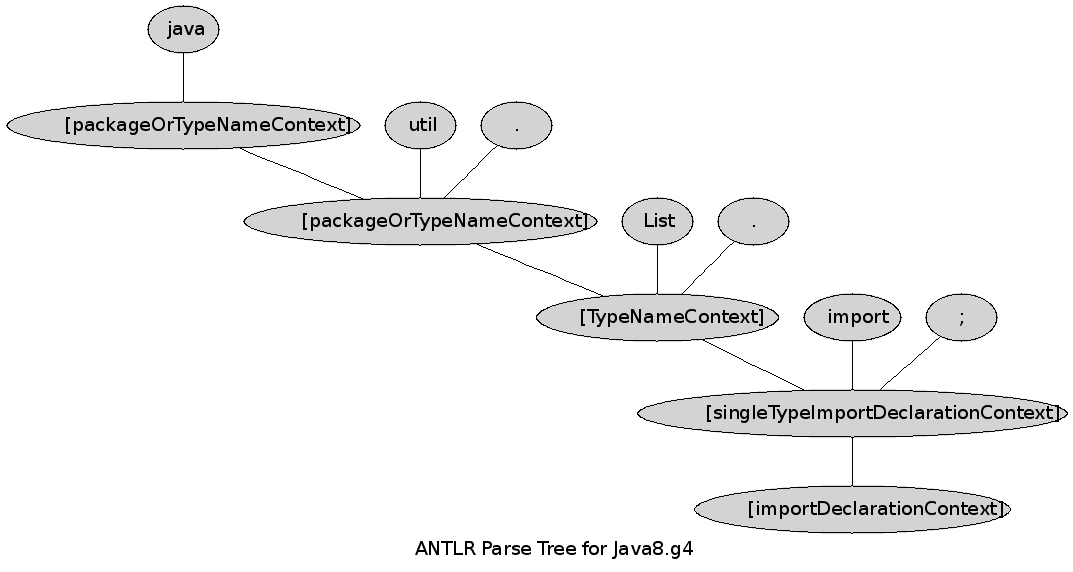
\includegraphics[width=.9\linewidth]{antlr-tree.png}

An easy way to review what our tree should look like is by adding a valid import statement to our test. It's pretty straightforward,
but there's one more thing we have to take care of. We need to find out how to build a subtree of "packageOrTypeNameContext" from our type.
But wait! Our grammar should handle that, we only need to parse our type, calling the "typeName" rule.

\begin{verbatim}
@Override
public CompilationUnitContext visitCompilationUnit(CompilationUnitContext ctx) {
    ImportDeclarationContext newImport = new ImportDeclarationContext(ctx, ctx.invokingState);
    SingleTypeImportDeclarationContext singleTypeImportDeclarationContext =
        new SingleTypeImportDeclarationContext(newImport, newImport.invokingState);
    newImport.addChild(singleTypeImportDeclarationContext);
    singleTypeImportDeclarationContext.addChild(new CommonToken(Java8Parser.IMPORT, "import"));
    Java8Lexer lexer = new Java8Lexer(new ANTLRInputStream(this.importType));
    CommonTokenStream tokens = new CommonTokenStream(lexer);
    Java8Parser parser = new Java8Parser(tokens);
    TypeNameContext typeNameContext = parser.typeName();
    singleTypeImportDeclarationContext.addChild(typeNameContext);
    newImport.addChild(new CommonToken(Java8Parser.COLON, ";"));

    ctx.addChild(newImport);
    return super.visitCompilationUnit(ctx);
}
\end{verbatim}

The test now passes, but when debugging I saw something suspicious: an error message was logged in the console, and one
node in the tree was referencing an exception. Then, reviewing the code, I decided it was much clearer if I let ANTLR
do the whole parsing, not just part of it.

\begin{verbatim}
@Override
public CompilationUnitContext visitCompilationUnit(CompilationUnitContext ctx) {
    ImportDeclarationContext newImport = new ImportDeclarationContext(ctx, ctx.invokingState);
    Java8Lexer lexer = new Java8Lexer(new ANTLRInputStream("import " + this.importType + ";"));
    CommonTokenStream tokens = new CommonTokenStream(lexer);
    Java8Parser parser = new Java8Parser(tokens);
    SingleTypeImportDeclarationContext singleTypeImportDeclaration = parser.singleTypeImportDeclaration();
    newImport.addChild(singleTypeImportDeclaration);

    ctx.addChild(newImport);
    return super.visitCompilationUnit(ctx);
}
\end{verbatim}

Now it's a little more readable, and it's parsing the import correctly with no complaints. But it still contains that redundant
ImportDeclarationContext object that we've made up for no reason. ANTLR can handle it if we start parsing one level higher.

\begin{verbatim}
@Override
public CompilationUnitContext visitCompilationUnit(CompilationUnitContext ctx) {
    Java8Lexer lexer = new Java8Lexer(new ANTLRInputStream("import " + this.importType + ";"));
    CommonTokenStream tokens = new CommonTokenStream(lexer);
    Java8Parser parser = new Java8Parser(tokens);
    ImportDeclarationContext newImport = parser.importDeclaration();

    ctx.addChild(newImport);
    return super.visitCompilationUnit(ctx);
}
\end{verbatim}

Now it's much better. Let's hope it's not too expensive in terms of performance. Clearly, we should reuse the lexer and tokens from the initial parsing stage. We'll fix it
when time is ready.

\subsubsection{Fifth test: Generating code}
\label{sec-1-3-5}

So far we've got ourselves familiar with the first two steps in the process: reading source code, and manipulating it. Now it's time to
work on generating code from an AST.

Needless to say, we'll use StringTemplate. It's the natural counterpart of ANTLR, it is easy to learn, and promotes good habits.
In our situation, we are trying to answer the question "how can I generate Java sources?", but that's overly ambitious for a
first test.

On the top of my mind, I dream of finding a way to somehow mirror a grammar automatically. Let's consider the following rules from our grammar:

\begin{verbatim}
packageDeclaration
      :	packageModifier* 'package' Identifier ('.' Identifier)* ';'
      ;

packageModifier
      :	annotation
      ;

annotation
      :	normalAnnotation
      |	markerAnnotation
      |	singleElementAnnotation
      ;

normalAnnotation
      :	'@' typeName '(' elementValuePairList? ')'
      ;

markerAnnotation
      :	'@' typeName
      ;

singleElementAnnotation
      :	'@' typeName '(' elementValue ')'
      ;

typeName
      :	Identifier
      |	packageOrTypeName '.' Identifier
      ;

packageOrTypeName
      :	Identifier
      |	packageOrTypeName '.' Identifier
      ;

elementValuePairList
      :	elementValuePair (',' elementValuePair)*
      ;

elementValuePair
      :	Identifier '=' elementValue
      ;

elementValue
      :	conditionalExpression
      |	elementValueArrayInitializer
      |	annotation
      ;
\end{verbatim}

We could think of analogous StringTemplate rules:

\begin{verbatim}
packageDeclaration(modifiers, identifier, extraIdentifiers) ::= <<
<modifiers:{ m | <packageModifier(mod=m)>}; separator=" "> package <identifier><extraIdentifiers:{ e | .<e>}>;
>>

packageModifier(mod) ::= <<
<annotation(a=mod)>
>>

annotation(a) ::= <<
<if(a.normal)><
  normalAnnotation(a=a)><
else><
  if(a.marker)><
    markerAnnotation(a=a)><
  else><
    singleElementAnnotation(a=a)><
  endif><
endif>
>>

normalAnnotation(a) ::= <<
@<typeName(i=a)>(<if(a.elementValuePairList)><a.elementValuePairList:{ p |<elementValuePairList(pair=p)>}><endif>)
>>

markerAnnotation(a) ::= <<
@<typeName(i=a)>
>>

singleElementAnnotation(a) ::= <<
@<typeName(i=a)>(<a.elementValue>)
>>

typeName(i, p) ::= <<
<if(p)><p>.<i><else><i><endif>
>>

packageOrTypeName(i, p) ::= << <! it's the same as typeName !>
<if(p)><p>.<i><else><i><endif>
>>

elementValuePairList(pair) ::= <<
<pair:{ p |<elementValuePair(i=p.identifier, v=p.elementValue)>}; separator=",">
>>

elementValuePair(p, v) ::= <<
<i>=<elementValue(v=v)>
>>

elementValue(v) ::= <<
<if(v.conditionalExpression)><
  conditionalExpression(e=v)><
else><
  if(v.elementValueArrayInitializer)><
    elementValueArrayInitializer(i=v)><
  else><
    annotation(a=v)><
  endif><
endif>
>>
\end{verbatim}

I hope you get the idea. There seems to exist an automatically-generated template set for a given ANTLR grammar, given the AST/ParseTree
provides getters for each subtree, so StringTemplate can access them.
But don't have that ANTLR->StringTemplate conversion, and still we want to generate code from a AST modelling a Java source file.
I see two options: either build that tool ourselves, or build the StringTemplate templates we need for our particular purpose.
Let's explore both options in detail.

\begin{itemize}
\item Option A: Build an ANTLR->StringTemplate translator
\end{itemize}

We're pretty confident that, for a clean (no semantic predicates, no embedded logic) ANTLR grammar, there exist a
set of StringTemplate templates which can generate valid input for such grammar.

Such translator would involve:
a) An ANTLR meta-parser, which reads an ANTLR grammar and generates the StringTemplate templates.
b) An AST runtime decorator, which lets StringTemplate access the child nodes via getters.

\begin{itemize}
\item Option B: Hand-code the templates for Java8.g4
\end{itemize}

We've already felt the pain, above. Counting the parser rules gives us an astounding 271 rules. Of course, we could
reduce that number to certain extent. But it's a lot of work indeed. Besides that, our work is not usable for other languages
in the future, and forces us maintaining the generator manually.

So given this scenario, what would you decide? Each option has pros and cons. If we apply Lean philosophy, we should try to
obtain feedback as soon as possible, regardless of the option. Under that perspective, let's review the actual hypothesis behind
each option.

\begin{itemize}
\item Hypothesis for A: the automatic generation is feasible for any grammar, given it doesn't include logic or semantic predicates.
\end{itemize}

How could we possibly validate the hypothesis? If it doesn't hold, the whole point of building a generator is unclear. We can inspect
some grammars already available for ANTLR, to check for some situations which were not anticipated.

\begin{itemize}
\item Hypothesis for B: A custom generator for Java8.g4 is doable for sure, but it'll take a lot of time, and we'll have to write tests for
\end{itemize}
lots of language constructs.

How long would it be? Hours? Days? We could implement just the templates above, for the "package" rule, and with that information
try to estimate the whole grammar.

\subsection{Pivoting the prototype}
\label{sec-1-4}

We could discuss each of the options endlessly, and still miss the important challenge we are actually facing. We want to implement
a way to customize certain aspects and behavior of the generation templates, ortogonally to the templates themselves. It makes
much more sense to focus on that particular problem, than whether we can automate default templates from grammars.

\subsubsection{Background}
\label{sec-1-4-1}

Let's start with the same template to output Java package declarations:

packageDeclaration(modifiers, identifier, extraIdentifiers) ::= <<
<modifiers:\{ m | <packageModifier(mod=m)>\}; separator=" "> package <identifier><extraIdentifiers:\{ e | .<e>\}>;
>>

That template is saying:
\begin{itemize}
\item If there're any package modifiers, then run the "packageModifier" template for each of them, using a blank space
\end{itemize}
as separator.
\begin{itemize}
\item Append a blank space.
\item Add the "package" word.
\item Append the identifier value.
\item If there're any extra identifiers (the package is part of a tree), then append each part, preceded by a dot.
\item Append a semicolon.
\item Append a new line.
\end{itemize}

We'd like to be able to change how the template behaves:
\begin{itemize}
\item The separator used when calling "packageModifier" templates.
\item The blank space.
\item The "package" word.
\item The identifier value.
\item The separator used when calling the anonymous template.
\item The semicolon.
\item The new line.
\end{itemize}

Let's try to define selectors for each one of the identified elements:
\begin{itemize}
\item .packageDeclaration .packageModifiers : To overwrite the "separator" directive.
\item .packageDeclaration "package"::before : To tune the blank space before the "package".
\item .packageDeclaration \#identifier : to modify the way the identifier value is printed.
\item .packageDeclaration \#extraIdentifiers : again, needed to overwrite the separator.
\item .packageDeclaration ";"::before : to optionally add text before the semicolon.
\item .packageDeclaration ";" "s*" : to change whether there's a new line after the semicolon.
\end{itemize}

This is just an initial example, trying to adapt the standard \href{http://www.w3.org/TR/2011/REC-css3-selectors-20110929/}{CSS selectors} to this scenario. What we are doing here is
modeling the template itself as a DOM or AST, and filtering certain nodes or properties of such tree. But before worrying
about that, we need to implement a DSL for the new CSS-like grammar. And that requires us to go on with our initial
outline of what we'd like to build.

The next piece in the puzzle is defining the CSS-like properties to apply to the nodes matched by the selectors.
If we wanted to use two spaces after the "package" word, and two new lines after the semicolon, we would write it as follows:

\begin{verbatim}
.packageDeclaration #identifier::before {
  content: "  ";
}

.packageDeclaration ";"::after {
  content: "[newline][newline]";
}
\end{verbatim}

CSS Text defines certain properties we could reuse, but only to a certain extent, since their meaning and units are
not compatible in some cases.

Anyway, let's try to implement such DSL, starting with a test.

\subsubsection{First test: Parsing the CSS-like DSL}
\label{sec-1-4-2}

This first test consists of invoking logic on a new StringTemplateCSSParser class to parse the above examples. The output
will consist of a list, and a map of maps. A list since the selectors are an ordered collection of items, with precedence semantics.
A map since the properties are a flattened JSON-like structure of key-value tuples.

\begin{verbatim}
@Test
public void parses_a_simple_input() {
    String input =
        ".packageDeclaration #identifier::before {\n"
      + "    content: \"  \";\n"
      + "}\n";

    StringTemplateCSSLexer lexer =
        new StringTemplateCSSLexer(
            new ANTLRInputStream(input));

    CommonTokenStream tokens = new CommonTokenStream(lexer);

    StringTemplateCSSParser parser =
        new StringTemplateCSSParser(tokens);
    ParseTree ast = parser.css();
    Assert.assertNotNull(ast);
}
\end{verbatim}

As for the grammar itself, we can reuse the Java8 one, removing almost all the parser rules, and keeping the some of the lexer
ones.

\begin{verbatim}
css
     :	selector+ '{' property+ '}' EOF
     ;

selector
     :	('.' | '#') Identifier (':' ':' ('before' | 'after'))?
     ;

property
     :	Identifier ':' StringLiteral ';'
     ;

StringLiteral
     :	'"' StringCharacters? '"' | '\'' StringCharacters? '\''
     ;

fragment
StringCharacters
     :	StringCharacter+
     ;

fragment
StringCharacter
     :	~["\\]
     |	EscapeSequence
     ;

// §3.10.6 Escape Sequences for Character and String Literals

fragment
EscapeSequence
     :	'\\' [btnfr"'\\]
     |	OctalEscape
   |   UnicodeEscape // This is not in the spec but prevents having to preprocess the input
     ;

fragment
OctalEscape
     :	'\\' OctalDigit
     |	'\\' OctalDigit OctalDigit
     |	'\\' ZeroToThree OctalDigit OctalDigit
     ;

fragment
OctalDigit
     :	[0-7]
     ;

fragment
ZeroToThree
     :	[0-3]
     ;

// This is not in the spec but prevents having to preprocess the input
fragment
UnicodeEscape
    :   '\\' 'u' HexDigit HexDigit HexDigit HexDigit
    ;

fragment
HexDigit
     :	[0-9a-fA-F]
     ;

LBRACE : '{';
RBRACE : '}';
LBRACK : '[';
RBRACK : ']';
SEMI : ';';
COMMA : ',';
DOT : '.';

GT : '>';
LT : '<';
TILDE : '~';
COLON : ':';
MUL : '*';
COLONCOLON : '::';

// §3.8 Identifiers (must appear after all keywords in the grammar)

Identifier
     :	JavaLetter JavaLetterOrDigit*
     ;

fragment
JavaLetter
     :	[a-zA-Z$_] // these are the "java letters" below 0xFF
     |	// covers all characters above 0xFF which are not a surrogate
   	     ~[\u0000-\u00FF\uD800-\uDBFF]
   	     {Character.isJavaIdentifierStart(_input.LA(-1))}?
     |	// covers UTF-16 surrogate pairs encodings for U+10000 to U+10FFFF
   	     [\uD800-\uDBFF] [\uDC00-\uDFFF]
   	     {Character.isJavaIdentifierStart(Character.toCodePoint((char)_input.LA(-2), (char)_input.LA(-1)))}?
     ;

fragment
JavaLetterOrDigit
     :	[a-zA-Z0-9$_] // these are the "java letters or digits" below 0xFF
     |	// covers all characters above 0xFF which are not a surrogate
   	     ~[\u0000-\u00FF\uD800-\uDBFF]
   	     {Character.isJavaIdentifierPart(_input.LA(-1))}?
     |	// covers UTF-16 surrogate pairs encodings for U+10000 to U+10FFFF
   	     [\uD800-\uDBFF] [\uDC00-\uDFFF]
   	     {Character.isJavaIdentifierPart(Character.toCodePoint((char)_input.LA(-2), (char)_input.LA(-1)))}?
     ;

AT : '@';
ELLIPSIS : '...';

//
// Whitespace and comments
//

WS  :  [ \t\r\n\u000C]+ -> skip
    ;

COMMENT
    :   '/*' .*? '*/' -> skip
    ;

LINE_COMMENT
    :   '//' ~[\r\n]* -> skip
    ;
\end{verbatim}

Our test succeeds. We can live with that "Java" rules in the lexer, since they probably hold true for the CSS
specification we are trying to emulate as accurate as possible.

Let's check if the other input we wrote before is parsed correctly as well:

\begin{verbatim}
@Test
public void parses_another_simple_input() {
    String input =
          "  .packageDeclaration \";\"::after {\n"
        + "    content: \"\\n\\n\";\n"
        + "  }";

    StringTemplateCSSLexer lexer =
        new StringTemplateCSSLexer(
            new ANTLRInputStream(input));

    CommonTokenStream tokens = new CommonTokenStream(lexer);

    StringTemplateCSSParser parser =
        new StringTemplateCSSParser(tokens);
    ParseTree ast = parser.css();
    Assert.assertNotNull(ast);
}
\end{verbatim}

The test passes, but ANTLR complains in the console. There're two issues: first, the grammar is not parsing the input correctly; second, the test (and the previous one as well) doesn't
detect when the parsing is failing.

\begin{verbatim}
Running org.acmsl.javacss.css.parser.StringTemplateCSSParserTest
line 1:31 extraneous input '::' expecting {'#', '{', '.'}
line 1:22 extraneous input '";"' expecting {'#', '{', '.'}
Tests run: 2, Failures: 0, Errors: 0, Skipped: 0, Time elapsed: 0.004 sec - in org.acmsl.javacss.css.parser.StringTemplateCSSParserTest
\end{verbatim}

For now, it's more important to fix the tests. Changing the ErrorHandler to a less permissive strategy is exactly what we look for.

\begin{verbatim}
parser.setErrorHandler(new BailErrorStrategy());
\end{verbatim}

Now the tests fail as they should, we deal with why the grammar doesn't expect "::" in the first test. The second part of the selector, \#identifier::before, is not a valid selector according to our grammar.
The problem was that we described the consecutive colons as two tokens, whereas the lexer identified them as COLONCOLON:

\begin{verbatim}
selector
     :	('.' | '#') Identifier (COLONCOLON ('before' | 'after'))?
     ;
\end{verbatim}

That fixes the first test. The second input is clearly not supported by our current grammar. We'll need to implement it, but it is not difficult.

\begin{verbatim}
selector
     :	('.' | '#')? (Identifier | StringLiteral) (COLONCOLON ('before' | 'after'))?
     ;
\end{verbatim}

\subsubsection{Second test: Listing selectors}
\label{sec-1-4-3}

Next, we want to define how to list all selectors defined. As before, we'll start with a simple helper which uses
the ANTLR-generated parser and provides the two collections we need: the list of selectors, and a Map of Maps containing the properties for each selector.
We'll envelop this in a StringTemplateCSSHelper class for now.

\begin{verbatim}
@Test
public void retrieves_selectors_for_a_simple_input()
{
    String input =
        ".packageDeclaration #identifier::before {\n"
        + "    content: \"  \";\n"
        + "}\n";

    StringTemplateCSSHelper helper = new StringTemplateCSSHelper(input);

    List<String> selectors = helper.getSelectors();

    Assert.assertNotNull(selectors);

    Assert.assertEquals(1, selectors.size());

    Assert.assertEquals(".packageDeclaration #identifier::before", selectors.get(0));
}
\end{verbatim}

We can now proceed writing the skeleton of the class to ensure the code compiles.

\begin{verbatim}
public class StringTemplateCSSHelper
{
    private final String input;
    private List<String> selectors = new ArrayList<String>();

    public StringTemplateCSSHelper(final String input)
    {
        this.input = input;
    }

    public List<String> getSelectors()
    {
        return this.selectors;
    }
}
\end{verbatim}

Now that we have our beloved red light, we can try to implement the logic. Notice I'm bypassing the "dumb" implementation here. Anyway, my first attempt wasn't much better either.

\begin{verbatim}
public List<String> getSelectors()
{
    if (this.selectors == null)
    {
        initialize(this.input);
    }

    return this.selectors;
}

protected void initialize(String input)
{
    StringTemplateCSSLexer lexer = new StringTemplateCSSLexer(new ANTLRInputStream(input));

    CommonTokenStream tokens = new CommonTokenStream(lexer);

    StringTemplateCSSParser parser = new StringTemplateCSSParser(tokens);

    ParseTree tree = parser.css();

    Collection<ParseTree> selectorEntries = XPath.findAll(tree, "//selector", parser);

    this.selectors = new ArrayList<String>(selectorEntries.size());

    for (ParseTree selectorEntry : selectorEntries)
    {
        this.selectors.add(selectorEntry.getText());
    }
}
\end{verbatim}

The test doesn't pass because it expects just one selector, and the helper is returning two. And we're returning two
because it's what the grammar dictates. For now, I feel more confortable with the idea that each block belongs
to one selector, even though it's not really true. It's the combination of selectors (and some relationships among them) what allow us
to match certain pieces of each template. But again, we'll leave that for later. Meanwhile, let's update the grammar to
wrap all selectors into one.

\begin{verbatim}
css
     :	selectorCombination '{' property+ '}' EOF
     ;

selectorCombination
     :	selector+
     ;
\end{verbatim}

Voilà! It did the trick, although the test is not passing yet, but this time is the test's fault.

\begin{verbatim}
retrieves_selectors_for_a_simple_input(org.acmsl.javacss.css.StringTemplateCSSHelperTest)  Time elapsed: 0.002 sec  <<< FAILURE!
org.junit.ComparisonFailure: expected:<.packageDeclaration[ ]#identifier::before> but was:<.packageDeclaration[]#identifier::before>
        at org.junit.Assert.assertEquals(Assert.java:115)
        at org.junit.Assert.assertEquals(Assert.java:144)
        at org.acmsl.javacss.css.StringTemplateCSSHelperTest.retrieves_selectors_for_a_simple_input(StringTemplateCSSHelperTest.java:70)
\end{verbatim}

In our test, we are calling getText() on non-terminal nodes of our ParseTree. In our grammar the whitespace is not meaningful, so it's
discarded by the lexer and omitted in the token stream and in the final tree. Therefore it's not returning the same input text, and
we have to take it into account in our checks.

\begin{verbatim}
@Test
public void retrieves_selectors_for_a_simple_input()
{
    [..]

    Assert.assertEquals(".packageDeclaration#identifier::before", selectors.get(0));
}
\end{verbatim}

We should extend this test to verify it is prepared for input containing more than one block.

It's easy to make the test generic and don't assume a fixed number of blocks, at the cost of making
the test non-deterministic.

\begin{verbatim}
protected void multipleBlockTests(int count)
{
    StringBuilder input =
        new StringBuilder(".packageDeclaration #identifier");

    for (int index = 0; index < count; index++)
    {
        input.append("::before {\n    content: \"  \";\n}\n");
    }

    StringTemplateCSSHelper helper = new StringTemplateCSSHelper(input.toString());

    List<String> selectors = helper.getSelectors();

    Assert.assertNotNull(selectors);

    Assert.assertEquals(count, selectors.size());

    for (int index = 0; index < count; index++)
    {
        Assert.assertEquals(".packageDeclaration#identifier" + index + "::before", selectors.get(index));
    }
}

@Test
public void retrieves_selectors_for_an_input_with_several_blocks()
{
    multipleBlockTests((int) (Math.random() * 10));
}
\end{verbatim}

However, the input we are building to test our helper is not valid. It generates texts like

\begin{verbatim}
.packageDeclaration #identifier::before {
    content: "  ";
}

::before {
    content: "  ";
}
\end{verbatim}

I forgot the ".packageDeclaration \#identifier" part, and we'd better off appending the count to make rules different from each another.

\begin{verbatim}
protected void multipleBlockTests(int count)
{
    StringBuilder input = new StringBuilder();

    for (int index = 0; index < count; index++)
    {
        input.append(".packageDeclaration #identifier");
        input.append(index);
        input.append("::before {\n    content: \"  \";\n}\n\n");
    }

    StringTemplateCSSHelper helper = new StringTemplateCSSHelper(input.toString());

    List<String> selectors = helper.getSelectors();

    Assert.assertNotNull(selectors);

    Assert.assertEquals(count, selectors.size());

    for (int index = 0; index < count; index++)
    {
        Assert.assertEquals(".packageDeclaration#identifier" + index + "::before", selectors.get(index));
    }
}
\end{verbatim}

Now some tests pass, some doesn't. For a count of 2 it doesn't work. Let's force that test to dig into the issue. The input we are parsing is:

\begin{verbatim}
.packageDeclaration #identifier0::before {
    content: "  ";
}

.packageDeclaration #identifier1::before {
    content: "  ";
}
\end{verbatim}

Here's the mismatched input error: 

Running org.acmsl.javacss.css.parser.StringTemplateCSSParserTest
line 5:0 mismatched input '.' expecting <EOF>

If we review our grammar, the problem is obvious. The "css" rule is expecting just one block, so let's make it recursive.

\begin{verbatim}
css
       :	selectorCombination '{' property+ '}' css* EOF
       ;
\end{verbatim}

Now it works, so let's revert the test to a random number of blocks.

Our current "multipleBlockTests" method should be "multipleBlockSelectorTests" instead, so let's change that first.

\begin{verbatim}
protected void multipleBlockSelectorTests(int count)
{
    [..]
}
\end{verbatim}


\subsubsection{Third test: Reading properties}
\label{sec-1-4-4}

Next, we want to define how to retrieve the properties associated to a selector. A basic test would simply ask for all properties contained in a block, and verify its contents. 

\begin{verbatim}
@Test
public void retrieves_properties_for_a_simple_input()
{
    String input =
        ".packageDeclaration #identifier::before {\n"
        + "    content: \"  \";\n"
        + "}\n";

    StringTemplateCSSHelper helper = new StringTemplateCSSHelper(input);

    List<String> selectors = helper.getSelectors();

    Assert.assertNotNull(selectors);

    Assert.assertEquals(1, selectors.size());

    Map<String, String> properties = helper.getProperties(selectors.get(0));

    Assert.assertNotNull(properties);

    Assert.assertEquals(1, properties.size());

    Assert.assertTrue(properties.containsKey("content"));
    Assert.assertEquals("  ", properties.get("content"));
}
\end{verbatim}

As always, we need to provide the skeleton to make it compile.

\begin{verbatim}
public Map<String, String> getProperties(String selector)
{
    return null;
}
\end{verbatim}

As expected, the test fails.

\begin{verbatim}
Tests run: 3, Failures: 1, Errors: 0, Skipped: 0, Time elapsed: 0.001 sec <<< FAILURE! - in org.acmsl.javacss.css.StringTemplateCSSHelperTest
retrieves_properties_for_a_simple_input(org.acmsl.javacss.css.StringTemplateCSSHelperTest)  Time elapsed: 0 sec  <<< FAILURE!
java.lang.AssertionError: null
        at org.junit.Assert.fail(Assert.java:86)
        at org.junit.Assert.assertTrue(Assert.java:41)
        at org.junit.Assert.assertNotNull(Assert.java:621)
        at org.junit.Assert.assertNotNull(Assert.java:631)
        at org.acmsl.javacss.css.StringTemplateCSSHelperTest.retrieves_properties_for_a_simple_input(StringTemplateCSSHelperTest.java:123)
\end{verbatim}

My first attempt to implement this was:

\begin{verbatim}
private Map<String, Map<String, String>> properties;

[..]

protected void initialize(String input)
{
    StringTemplateCSSLexer lexer = new StringTemplateCSSLexer(new ANTLRInputStream(input));

    CommonTokenStream tokens = new CommonTokenStream(lexer);

    StringTemplateCSSParser parser = new StringTemplateCSSParser(tokens);

    ParseTree tree = parser.css();

    Collection<ParseTree> selectorEntries = XPath.findAll(tree, "//selectorCombination", parser);

    this.selectors = new ArrayList<String>(selectorEntries.size());
    this.properties = new HashMap<String, Map<String, String>>();

    for (ParseTree selectorEntry : selectorEntries)
    {
        String text = selectorEntry.getText();
        this.selectors.add(text);
        Map<String, String> block = retrieveProperties(selectorEntry, parser);

        this.properties.put(text, block);
    }
}

protected Map<String, String> retrieveProperties(ParseTree selectorEntry, StringTemplateCSSParser parser)
{
    Map<String, String> result;

    Collection<ParseTree> properties = XPath.findAll(selectorEntry, "//property", parser);

    result = new HashMap<String, String>(properties.size());

    for (ParseTree property : properties)
    {
        String key = property.getChild(0).getText();
        String value = property.getChild(2).getText();
        result.put(key, value);
    }

    return result;
}

public Map<String, String> getProperties(String selector)
{
    if (this.properties == null)
    {
        initialize(this.input);
    }

    return this.properties.get(selector);
}
\end{verbatim}

However, it didn't make the test pass.

\begin{verbatim}
Tests run: 3, Failures: 1, Errors: 0, Skipped: 0, Time elapsed: 0.006 sec <<< FAILURE! - in org.acmsl.javacss.css.StringTemplateCSSHelperTest
retrieves_properties_for_a_simple_input(org.acmsl.javacss.css.StringTemplateCSSHelperTest)  Time elapsed: 0.006 sec  <<< FAILURE!
java.lang.AssertionError: expected:<1> but was:<0>
        at org.junit.Assert.fail(Assert.java:88)
        at org.junit.Assert.failNotEquals(Assert.java:743)
        at org.junit.Assert.assertEquals(Assert.java:118)
        at org.junit.Assert.assertEquals(Assert.java:555)
        at org.junit.Assert.assertEquals(Assert.java:542)
        at org.acmsl.javacss.css.StringTemplateCSSHelperTest.retrieves_properties_for_a_simple_input(StringTemplateCSSHelperTest.java:125)
\end{verbatim}

The reason is that our XPath expression, "//property", is not finding anything. If we review the code, we can figure out why: the first argument to the "retrieveProperties()" should be the "css" node, and we are passing the "selectorCombination" node.
A simple change to passing "selectorEntry.getParent()" allows the block to be parsed successfully.

\begin{verbatim}
protected void initialize(String input)
{
    StringTemplateCSSLexer lexer = new StringTemplateCSSLexer(new ANTLRInputStream(input));

    CommonTokenStream tokens = new CommonTokenStream(lexer);

    StringTemplateCSSParser parser = new StringTemplateCSSParser(tokens);

    ParseTree tree = parser.css();

    Collection<ParseTree> selectorEntries = XPath.findAll(tree, "//selectorCombination", parser);

    this.selectors = new ArrayList<String>(selectorEntries.size());
    this.properties = new HashMap<String, Map<String, String>>();

    for (ParseTree selectorEntry : selectorEntries)
    {
        String text = selectorEntry.getText();
        this.selectors.add(text);
        Map<String, String> block = retrieveProperties(selectorEntry.getParent(), parser);

        this.properties.put(text, block);
    }
}

protected Map<String, String> retrieveProperties(ParseTree cssEntry, StringTemplateCSSParser parser)
{
    Map<String, String> result;

    Collection<ParseTree> properties = XPath.findAll(cssEntry, "//property", parser);

    result = new HashMap<String, String>(properties.size());

    for (ParseTree property : properties)
    {
        String key = property.getChild(0).getText();
        String value = property.getChild(2).getText();
        result.put(key, value);
    }

    return result;
}

public Map<String, String> getProperties(String selector)
{
    if (this.properties == null)
    {
        initialize(this.input);
    }

    return this.properties.get(selector);
}
\end{verbatim}

But the test still fails.

\begin{verbatim}
retrieves_properties_for_a_simple_input(org.acmsl.javacss.css.StringTemplateCSSHelperTest)  Time elapsed: 0.001 sec  <<< FAILURE!
org.junit.ComparisonFailure: expected:<[  ]> but was:<["  "]>
        at org.junit.Assert.assertEquals(Assert.java:115)
        at org.junit.Assert.assertEquals(Assert.java:144)
        at org.acmsl.javacss.css.StringTemplateCSSHelperTest.retrieves_properties_for_a_simple_input(StringTemplateCSSHelperTest.java:128)
\end{verbatim}

We have two options. Process the value of each property to remove any surrounding quotes, or leave them as they are, and update the test. Since we are not dealing with the nature of the property values, I can live with a test assuming the values can be quoted until it's time to focus on the property values.

\begin{verbatim}
Assert.assertEquals("\"  \"", properties.get("content"));
\end{verbatim}

As we did previously, let's make sure the properties are parsed correctly if the input contains several blocks. Also, we're interested in verifying the properties are specific for each block.

\begin{verbatim}
protected void multipleBlockPropertyTests(int count)
{
    StringBuilder input = new StringBuilder();

    for (int index = 0; index < count; index++)
    {
        input.append(".packageDeclaration #identifier");
        input.append(index);
        input.append("::before {\n");
        input.append("    content: \"");
        input.append(index);
        input.append("\";\n");
        input.append("}\n");
    }

    StringTemplateCSSHelper helper = new StringTemplateCSSHelper(input.toString());

    List<String> selectors = helper.getSelectors();

    Assert.assertNotNull(selectors);

    Assert.assertEquals(count, selectors.size());

    for (int index = 0; index < count; index++)
    {
        Map<String, String> properties = helper.getProperties(selectors.get(index));

        Assert.assertNotNull(properties);

        Assert.assertEquals(1, properties.size());

        Assert.assertTrue(properties.containsKey("content"));
        Assert.assertEquals("\"" + index + "\"", properties.get("content"));
    }
}

@Test
public void retrieves_properties_for_a_simple_input()
{
    multipleBlockPropertyTests(1);
}
\end{verbatim}

This new test is equilavent to the previous one, and passes. Let's check what happens for random number of blocks.

\begin{verbatim}
@Test
public void retrieves_properties_for_an_input_with_multiple_blocks()
{
    multipleBlockPropertyTests((int) (Math.random() * 10));
}
\end{verbatim}

It doesn't. It's a bit frustrating, but it also gives a great sense of progress.

\begin{verbatim}
Tests run: 4, Failures: 1, Errors: 0, Skipped: 0, Time elapsed: 0.007 sec <<< FAILURE! - in org.acmsl.javacss.css.StringTemplateCSSHelperTest
retrieves_properties_for_an_input_with_multiple_blocks(org.acmsl.javacss.css.StringTemplateCSSHelperTest)  Time elapsed: 0.007 sec  <<< FAILURE!
java.lang.AssertionError: expected:<0> but was:<1>
        at org.junit.Assert.fail(Assert.java:88)
        at org.junit.Assert.failNotEquals(Assert.java:743)
        at org.junit.Assert.assertEquals(Assert.java:118)
        at org.junit.Assert.assertEquals(Assert.java:555)
        at org.junit.Assert.assertEquals(Assert.java:542)
        at org.acmsl.javacss.css.StringTemplateCSSHelperTest.multipleBlockPropertyTests(StringTemplateCSSHelperTest.java:126)
        at org.acmsl.javacss.css.StringTemplateCSSHelperTest.retrieves_properties_for_an_input_with_multiple_blocks(StringTemplateCSSHelperTest.java:150)


Results :

Failed tests: 
  StringTemplateCSSHelperTest.retrieves_properties_for_an_input_with_multiple_blocks:150->multipleBlockPropertyTests:126 expected:<0> but was:<1>
\end{verbatim}

To make debugging simpler, it's better to return to a deterministic testing context.


\begin{verbatim}
    @Test
    public void retrieves_properties_for_an_input_with_multiple_blocks()
    {
//        multipleBlockPropertyTests((int) (Math.random() * 10));
        multipleBlockPropertyTests(2);
    }
\end{verbatim}

It still fails, so it's not depending on how many blocks, but only if there's more than one. We've been here already. Probably the input
the test builds is incorrect, but ANTLR is not complaining. After a debugging session, I found out the issue. It's a bug that was not
detected in previous tests: when we are retrieving all "property" nodes in the ParseTree, we use an XPath expresion "//property" on the
"css" root node. However, that collection is the same, regardless which "css" or block we are processing. So at runtime, we iterate
over the selectors, and then associate the properties. Due to this bug, and since in our test all keys are the same, all values get overriden in
each iteration. We have to retrieve just the properties belonging to the specific selector, and therefore the XPath.findAll() call is
not correct.
The logic should be: for a "selectorCombination" node, its associated "properties" are the next-to-the-right siblings of type "property".
We could write a specific test for that, but we'd probably need to use a mock framework to build the tree. On the other hand, we are
already building such trees in our tests. Let's assume that new logic is indirectly tested already.
Anyway, why don't we implement it using a Visitor pattern instead?

\begin{verbatim}
protected Map<String, String> retrieveProperties(ParseTree selectorEntry, StringTemplateCSSParser parser)
{
    Map<String, String> result;

    Collection<ParseTree> properties = findPropertyNodes(selectorEntry);

    result = new HashMap<String, String>(properties.size());

    for (ParseTree property : properties)
    {
        String key = property.getChild(0).getText();
        String value = property.getChild(2).getText();
        result.put(key, value);
    }

    return result;
}

protected Collection<ParseTree> findPropertyNodes(final ParseTree selectorEntry)
{
    ParseTree parent = selectorEntry.getParent();
    PropertyVisitor visitor = new PropertyVisitor();
    parent.accept(visitor);

    return visitor.properties;
}

public Map<String, String> getProperties(String selector)
{
    if (this.properties == null)
    {
        initialize(this.input);
    }

    return this.properties.get(selector);
}

protected static class PropertyVisitor
    extends StringTemplateCSSBaseVisitor<ParseTree>
{
    final List<ParseTree> properties = new ArrayList<ParseTree>();

    public PropertyVisitor(final ParseTree parent)
    {
        this.parent = parent;
    }

    @Override
    public ParseTree visitProperty(@NotNull final PropertyContext ctx)
    {
        this.properties.add(ctx);
        return super.visitProperty(ctx);
    }
}
\end{verbatim}

Unfortunately it still fails.

\begin{verbatim}
Tests run: 4, Failures: 1, Errors: 0, Skipped: 0, Time elapsed: 0.001 sec <<< FAILURE! - in org.acmsl.javacss.css.StringTemplateCSSHelperTest
retrieves_properties_for_an_input_with_multiple_blocks(org.acmsl.javacss.css.StringTemplateCSSHelperTest)  Time elapsed: 0.001 sec  <<< FAILURE!
org.junit.ComparisonFailure: expected:<"[0]"> but was:<"[1]">
        at org.junit.Assert.assertEquals(Assert.java:115)
        at org.junit.Assert.assertEquals(Assert.java:144)
        at org.acmsl.javacss.css.StringTemplateCSSHelperTest.multipleBlockPropertyTests(StringTemplateCSSHelperTest.java:137)
        at org.acmsl.javacss.css.StringTemplateCSSHelperTest.retrieves_properties_for_an_input_with_multiple_blocks(StringTemplateCSSHelperTest.java:151)


Results :

Failed tests:
  StringTemplateCSSHelperTest.retrieves_properties_for_an_input_with_multiple_blocks:151->multipleBlockPropertyTests:137 expected:<"[0]"> but was:<"[1]">
\end{verbatim}

The problem now is that in our current grammar, each "css" node becomes the parent of the next "css" node to the right. And that
layout makes our visitor end up visiting all "property" nodes. To fix this, there're two options: changing the node tree (the grammar), or
ensuring we filter out all "property" nodes whose parent is not matching the selector's. The latter is simpler, but more
expensive at runtime, though.

\begin{verbatim}
protected Map<String, String> retrieveProperties(ParseTree selectorEntry, StringTemplateCSSParser parser)
{
    Map<String, String> result;

    Collection<ParseTree> properties = findPropertyNodes(selectorEntry);

    result = new HashMap<String, String>(properties.size());

    for (ParseTree property : properties)
    {
        String key = property.getChild(0).getText();
        String value = property.getChild(2).getText();
        result.put(key, value);
    }

    return result;
}

protected Collection<ParseTree> findPropertyNodes(final ParseTree selectorEntry)
{
    ParseTree parent = selectorEntry.getParent();
    PropertyVisitor visitor = new PropertyVisitor(selectorEntry.getParent());
    parent.accept(visitor);

    return visitor.properties;
}

public Map<String, String> getProperties(String selector)
{
    if (this.properties == null)
    {
        initialize(this.input);
    }

    return this.properties.get(selector);
}

protected static class PropertyVisitor
    extends StringTemplateCSSBaseVisitor<ParseTree>
{
    final List<ParseTree> properties = new ArrayList<ParseTree>();
    final ParseTree parent;

    public PropertyVisitor(final ParseTree parent)
    {
        this.parent = parent;
    }

    @Override
    public ParseTree visitProperty(@NotNull final PropertyContext ctx)
    {
        if (ctx.getParent() == this.parent)
        {
            this.properties.add(ctx);
        }
        return super.visitProperty(ctx);
    }
}
\end{verbatim}

We're now back into the green zone, but don't forget we're not calling "multipleBlockPropertyTests()" with random values. When
switching back to relying to input composed of a random number of blocks, the test fails again.


\begin{verbatim}
Tests run: 4, Failures: 1, Errors: 0, Skipped: 0, Time elapsed: 0.008 sec <<< FAILURE! - in org.acmsl.javacss.css.StringTemplateCSSHelperTest
retrieves_properties_for_an_input_with_multiple_blocks(org.acmsl.javacss.css.StringTemplateCSSHelperTest)  Time elapsed: 0.008 sec  <<< FAILURE!
java.lang.AssertionError: expected:<0> but was:<1>
        at org.junit.Assert.fail(Assert.java:88)
        at org.junit.Assert.failNotEquals(Assert.java:743)
        at org.junit.Assert.assertEquals(Assert.java:118)
        at org.junit.Assert.assertEquals(Assert.java:555)
        at org.junit.Assert.assertEquals(Assert.java:542)
        at org.acmsl.javacss.css.StringTemplateCSSHelperTest.multipleBlockPropertyTests(StringTemplateCSSHelperTest.java:133)
        at org.acmsl.javacss.css.StringTemplateCSSHelperTest.retrieves_properties_for_an_input_with_multiple_blocks(StringTemplateCSSHelperTest.java:158)


Results :

Failed tests:
  StringTemplateCSSHelperTest.retrieves_properties_for_an_input_with_multiple_blocks:158->multipleBlockPropertyTests:133 expected:<0> but was:<1>
\end{verbatim}

This test is interesting, because it uncovers one aspect we are not dealing with: invalid inputs. The "multipleBlockPropertyTest()" method, when receiving a 0 as parameter, generates
invalid input. Consequently, the parser complaints. Surprisingly, the XPath expression returns a match consisting of an empty string.

For now, let's annotate this for the next iteration: manage errors in ANTLR parsers / deal with invalid input. Meanwhile we have
to ensure we are not testing empty or wrong inputs.

\begin{verbatim}
@Test
public void retrieves_properties_for_an_input_with_multiple_blocks()
{
    multipleBlockPropertyTests((int) (Math.random() * 10) + 1);
}
\end{verbatim}

\subsubsection{Fourth test: Matching selectors}
\label{sec-1-4-5}

The next logical step is to find all matching selectors, for a given AST. We'll use it in the context of StringTemplate templates, but
need not to be constrained to any specific AST.

It's worth reviewing our selector syntax:

\begin{itemize}
\item a rule starting with a dot matches node classes.
\item a rule starting with a hash identifies unique nodes.
\item a rule with surrounding quotes selects nodes whose text matches the rule text.
\item any optional pseudo-element (::before or ::after) do not customize the nodes themselves, but add new siblings.
\end{itemize}

What would be a good scenario for checking if a selector is matching the correct node in a given AST? As always, start by
something simple, and increase in complexity gradually.

For our AST, a good fit could be the one produced by parsing this package declaration:

package com.foo.bar;

That is,

\includegraphics[width=.9\linewidth]{package-dot.png}

For the CSS, this would be simple enough: add a blank space before the semicolon.

\begin{verbatim}
.packageDeclaration ";"::before {
   content: " ";
}
\end{verbatim}

Notice we're not testing whether the final output included the blank space before the semicolon.
For now, we only want to implement the logic to find out which CSS block applies to each node in the AST. Or even simpler:
testing every node has no matching selectors, but the semicolon. Additionally, since we have no immediate need for a better
design, we'll implement the logic in our current helper class.


\begin{verbatim}
@Test
public void finds_the_matching_selector()
{
    String javaInput = "package com.foo.bar;";

    String cssInput =
          ".packageDeclaration \";\"::before {\n"
        + "   content: \" \";\n"
        + "}\n";

    StringTemplateCSSHelper helper = new StringTemplateCSSHelper(cssInput);

    Java8Lexer lexer = new Java8Lexer(new ANTLRInputStream(javaInput));
    CommonTokenStream tokens = new CommonTokenStream(lexer);
    Java8Parser parser = new Java8Parser(tokens);
    ParseTree ast = parser.compilationUnit();

    Collection<ParseTree> matches = XPath.findAll(ast, "//';'", parser);

    Assert.assertNotNull(matches);
    Assert.assertEquals(1, matches.size());

    ParseTree semiColon = matches.toArray(new ParseTree[1])[0];
    Assert.assertNotNull(semiColon);

    String matchedSelectors = helper.retrieveMatchingSelectors(semiColon);

    Assert.assertNotNull(matchedSelectors);
    Assert.assertEquals(".packageDeclaration \";\"::before", matchedSelectors);
}
\end{verbatim}

This test is more involved, and of course it won't compile until we write the new method "retrieveMatchingSelectors()".

\begin{verbatim}
public String retrieveMatchingSelectors(ParseTree semiColon)
{
    return null;
}
\end{verbatim}

And as expected, the null assertion makes the test fail.

\begin{verbatim}
Tests run: 5, Failures: 1, Errors: 0, Skipped: 0, Time elapsed: 0.015 sec <<< FAILURE! - in org.acmsl.javacss.css.StringTemplateCSSHelperTest
finds_the_matching_selector(org.acmsl.javacss.css.StringTemplateCSSHelperTest)  Time elapsed: 0.007 sec  <<< FAILURE!
java.lang.AssertionError: null
        at org.junit.Assert.fail(Assert.java:86)
        at org.junit.Assert.assertTrue(Assert.java:41)
        at org.junit.Assert.assertNotNull(Assert.java:621)
        at org.junit.Assert.assertNotNull(Assert.java:631)
        at org.acmsl.javacss.css.StringTemplateCSSHelperTest.finds_the_matching_selector(StringTemplateCSSHelperTest.java:187)


Results :

Failed tests:
  StringTemplateCSSHelperTest.finds_the_matching_selector:187 null
\end{verbatim}

Now we have to actually implement the "retrieveMatchingSelectors()" method. It's not straight-forward: we
have to find which selector defines a set which includes the input AST. Currently, we are storing the combination of 
selectors as one piece of text. Parsing it again makes no sense whatsoever, so we should invest some time fixing this first.
Instead of a list of Strings, it makes more sense to describe it as a list of list of Strings.

\begin{verbatim}
public class StringTemplateCSSHelper
{
    private final String input;
    private List<List<String>> selectors;
    private Map<List<String>, Map<String, String>> properties;

    public StringTemplateCSSHelper(final String input)
    {
        this.input = input;
    }

    public List<List<String>> getSelectors()
    {
        if (this.selectors == null)
        {
            initialize(this.input);
        }

        return this.selectors;
    }

    protected void initialize(String input)
    {
        StringTemplateCSSLexer lexer = new StringTemplateCSSLexer(new ANTLRInputStream(input));

        CommonTokenStream tokens = new CommonTokenStream(lexer);

        StringTemplateCSSParser parser = new StringTemplateCSSParser(tokens);

        ParseTree tree = parser.css();

        Collection<ParseTree> selectorCombinations = XPath.findAll(tree, "//selectorCombination", parser);

        this.selectors = new ArrayList<List<String>>(selectorCombinations.size());
        this.properties = new HashMap<List<String>, Map<String, String>>();

        for (ParseTree selectorCombination : selectorCombinations)
        {
            List<String> currentSelectors = new ArrayList<String>(selectorCombination.getChildCount());
            this.selectors.add(currentSelectors);

            for (int index = 0; index < selectorCombination.getChildCount(); index++)
            {
                String text = selectorCombination.getChild(index).getText();
                currentSelectors.add(text);
            }
            Map<String, String> block = retrieveProperties(selectorCombination, parser);

            this.properties.put(currentSelectors, block);
        }
    }

    protected Map<String, String> retrieveProperties(ParseTree selectorEntry, StringTemplateCSSParser parser)
    {
        Map<String, String> result;

        Collection<ParseTree> properties = findPropertyNodes(selectorEntry);

        result = new HashMap<String, String>(properties.size());

        for (ParseTree property : properties)
        {
            String key = property.getChild(0).getText();
            String value = property.getChild(2).getText();
            result.put(key, value);
        }

        return result;
    }

    protected Collection<ParseTree> findPropertyNodes(final ParseTree selectorEntry)
    {
        ParseTree parent = selectorEntry.getParent();
        PropertyVisitor visitor = new PropertyVisitor(selectorEntry.getParent());
        parent.accept(visitor);

        return visitor.properties;
    }

    public Map<String, String> getProperties(List<String> selector)
    {
        if (this.properties == null)
        {
            initialize(this.input);
        }

        return this.properties.get(selector);
    }

    [..]
}
\end{verbatim}

The current StringTemplateCSSHelperTest needs to be modified because of the API changes.

\begin{verbatim}
    @Test
    public void retrieves_selectors_for_a_simple_input()
    {
        String input =
            ".packageDeclaration #identifier::before {\n"
            + "    content: \"  \";\n"
            + "}\n";

        StringTemplateCSSHelper helper = new StringTemplateCSSHelper(input);

        List<List<String>> selectorCombinations = helper.getSelectors();

        Assert.assertNotNull(selectorCombinations);

        Assert.assertEquals(1, selectorCombinations.size());

        List<String> selectors = selectorCombinations.get(0);
        Assert.assertEquals(2, selectors.size());

        Assert.assertEquals(".packageDeclaration", selectors.get(0));
        Assert.assertEquals("#identifier::before", selectors.get(1));
    }

    protected void multipleBlockSelectorTests(int count)
    {
        StringBuilder input = new StringBuilder();

        for (int index = 0; index < count; index++)
        {
            input.append(".packageDeclaration #identifier");
            input.append(index);
            input.append("::before {\n    content: \"  \";\n}\n\n");
        }

        StringTemplateCSSHelper helper = new StringTemplateCSSHelper(input.toString());

        List<List<String>> selectorCombinations = helper.getSelectors();

        Assert.assertNotNull(selectorCombinations);

        Assert.assertEquals(count, selectorCombinations.size());

        for (int index = 0; index < count; index++)
        {
            List<String> selectors = selectorCombinations.get(index);

            Assert.assertEquals(".packageDeclaration", selectors.get(0));
            Assert.assertEquals("#identifier" + index + "::before", selectors.get(1));
        }
    }

    @Test
    public void retrieves_selectors_for_an_input_with_several_blocks()
    {
        multipleBlockSelectorTests((int) (Math.random() * 10));
    }

    protected void multipleBlockPropertyTests(int count)
    {
        StringBuilder input = new StringBuilder();

        for (int index = 0; index < count; index++)
        {
            input.append(".packageDeclaration #identifier");
            input.append(index);
            input.append("::before {\n");
            input.append("    content: \"");
            input.append(index);
            input.append("\";\n");
            input.append("}\n");
        }

        StringTemplateCSSHelper helper = new StringTemplateCSSHelper(input.toString());

        List<List<String>> selectors = helper.getSelectors();

        Assert.assertNotNull(selectors);

        Assert.assertEquals(count, selectors.size());

        for (int index = 0; index < count; index++)
        {
            Map<String, String> properties = helper.getProperties(selectors.get(index));

            Assert.assertNotNull(properties);

            Assert.assertEquals(1, properties.size());

            Assert.assertTrue(properties.containsKey("content"));
            Assert.assertEquals("\"" + index + "\"", properties.get("content"));
        }
    }

    [..]
}
\end{verbatim}

Even though we've had to change the tests, the changes were pretty simple, and the test passed nicely.
% Emacs 24.4.1 (Org mode 8.2.10)
\end{document}
